\documentclass[a4paper]{article}

\usepackage[margin=2.5cm]{geometry}
\usepackage[pdftex]{graphicx}
\usepackage[utf8]{inputenc}
\usepackage[T1]{fontenc}
\usepackage{textcomp}
\usepackage{babel}
\usepackage{amsmath, amssymb}
\usepackage[colorlinks=true,linkcolor=blue]{hyperref}
\usepackage{float}
\usepackage{mathrsfs}
%\usepackage{enumitem}
%% for identity function 1:
\usepackage{bbm}
%%For category theory diagrams:
%\usepackage{tikz-cd}
%%For code (e.g. python) in latex:
%\usepackage{listings}
%
%Usage: 
%\begin{lstlisting}[language=Python]
%\end{lstlisting}

\newcommand{\incfig}[2][1]{%
\def\svgwidth{#1\columnwidth}
\import{./figures/}{#2.pdf_tex}
}


% figure support
\usepackage{import}
\usepackage{xifthen}
\pdfminorversion=7
\usepackage{pdfpages}
\usepackage{transparent}

\pdfsuppresswarningpagegroup=1

\setlength\parindent{0pt}

\newcommand{\qed}{\tag*{$\blacksquare$}}
\newcommand{\qedwhite}{\hfill \ensuremath{\Box}}

%Inequalities
\newcommand{\cycsum}{\sum_{\mathrm{cyc}}}
\newcommand{\symsum}{\sum_{\mathrm{sym}}}
\newcommand{\cycprod}{\prod_{\mathrm{cyc}}}
\newcommand{\symprod}{\prod_{\mathrm{sym}}}

%Linear Algebra

\DeclareMathOperator{\Span}{span}
\DeclareMathOperator{\Ima}{Im}
\DeclareMathOperator{\diag}{diag}
\DeclareMathOperator{\Ker}{Ker}
\DeclareMathOperator{\ob}{ob}
\DeclareMathOperator{\Hom}{Hom}
\DeclareMathOperator{\sk}{sk}
\DeclareMathOperator{\Vect}{Vect}
\DeclareMathOperator{\Set}{Set}
\DeclareMathOperator{\Group}{Group}
\DeclareMathOperator{\Ring}{Ring}
\DeclareMathOperator{\Ab}{Ab}
\DeclareMathOperator{\Top}{Top}
\DeclareMathOperator{\Htpy}{Htpy}
\DeclareMathOperator{\Cat}{Cat}
\DeclareMathOperator{\CAT}{CAT}
\DeclareMathOperator{\Cone}{Cone}


%Row operations
\newcommand{\elem}[1]{% elementary operations
\xrightarrow{\substack{#1}}%
}

\newcommand{\lelem}[1]{% elementary operations (left alignment)
\xrightarrow{\begin{subarray}{l}#1\end{subarray}}%
}

%SS
\DeclareMathOperator{\supp}{supp}
\DeclareMathOperator{\Var}{Var}

%NT
\DeclareMathOperator{\ord}{ord}

%Alg
\DeclareMathOperator{\Rad}{Rad}
\DeclareMathOperator{\Jac}{Jac}

\DeclareMathAlphabet{\pazocal}{OMS}{zplm}{m}{n}
\newcommand{\unif}{\pazocal{U}}

\begin{document}
    \textbf{20:} Use van Kampen's theorem to calculate the fundamental group of
    the double torus by dividing the surface into two halves, each of which is
    a punctured torus. Do the calculation again, this time splitting the
    surface into a disc and the closure of the complement of the disc.\\
    \linebreak
    \textit{Solution:}
    Using the usual identification space of the double torus and the
    triangulation from problem 1 on page 124 from homework 10 shown below:
    \begin{figure}[H]
        \centering
        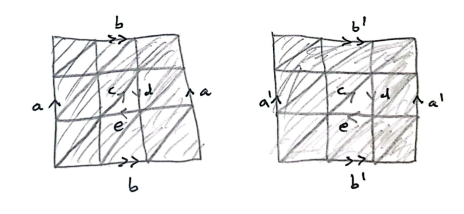
\includegraphics[width=0.6\textwidth]{1.png}
        \label{fig:1-png}
    \end{figure}
    we can let the left punctured torus be denoted by by $\left| J \right|
    $ and the right punctured torus be denoted by $\left| K \right| $.
    Then $\left| J \cap K \right| $ is $cde$ which is homeomorphic to
    a circle. Choose a basepoint $p$ on the circle
    $\left| J \cap K \right| $.\\
    Now, by problem 25 on page 109 from homework 9, the punctured torus has
    fundamental group isomorphic to the fundamental group of the one-point
    union of two circles, $S^{1} \vee S^{1}$, which, for example by example
    1 on page 136, has fundamental group $\mathbb{Z} * \mathbb{Z}$, the free
      group on two generators. Now, the inclusion of the circle
      $\left| J \cap K \right| $ in either  $\left| J \right| $ or $\left| K \right| $ 
      (equivalent by symmetry) is the circle constituting the border of the
      puncture. Now, considering the deformation retraction given in problem 25
      on homework 9, this circle corresponds the loop around the edges, given
      by
      $ab a^{-1}b^{-1}$ as shown below
      \begin{figure}[H]
          \centering
          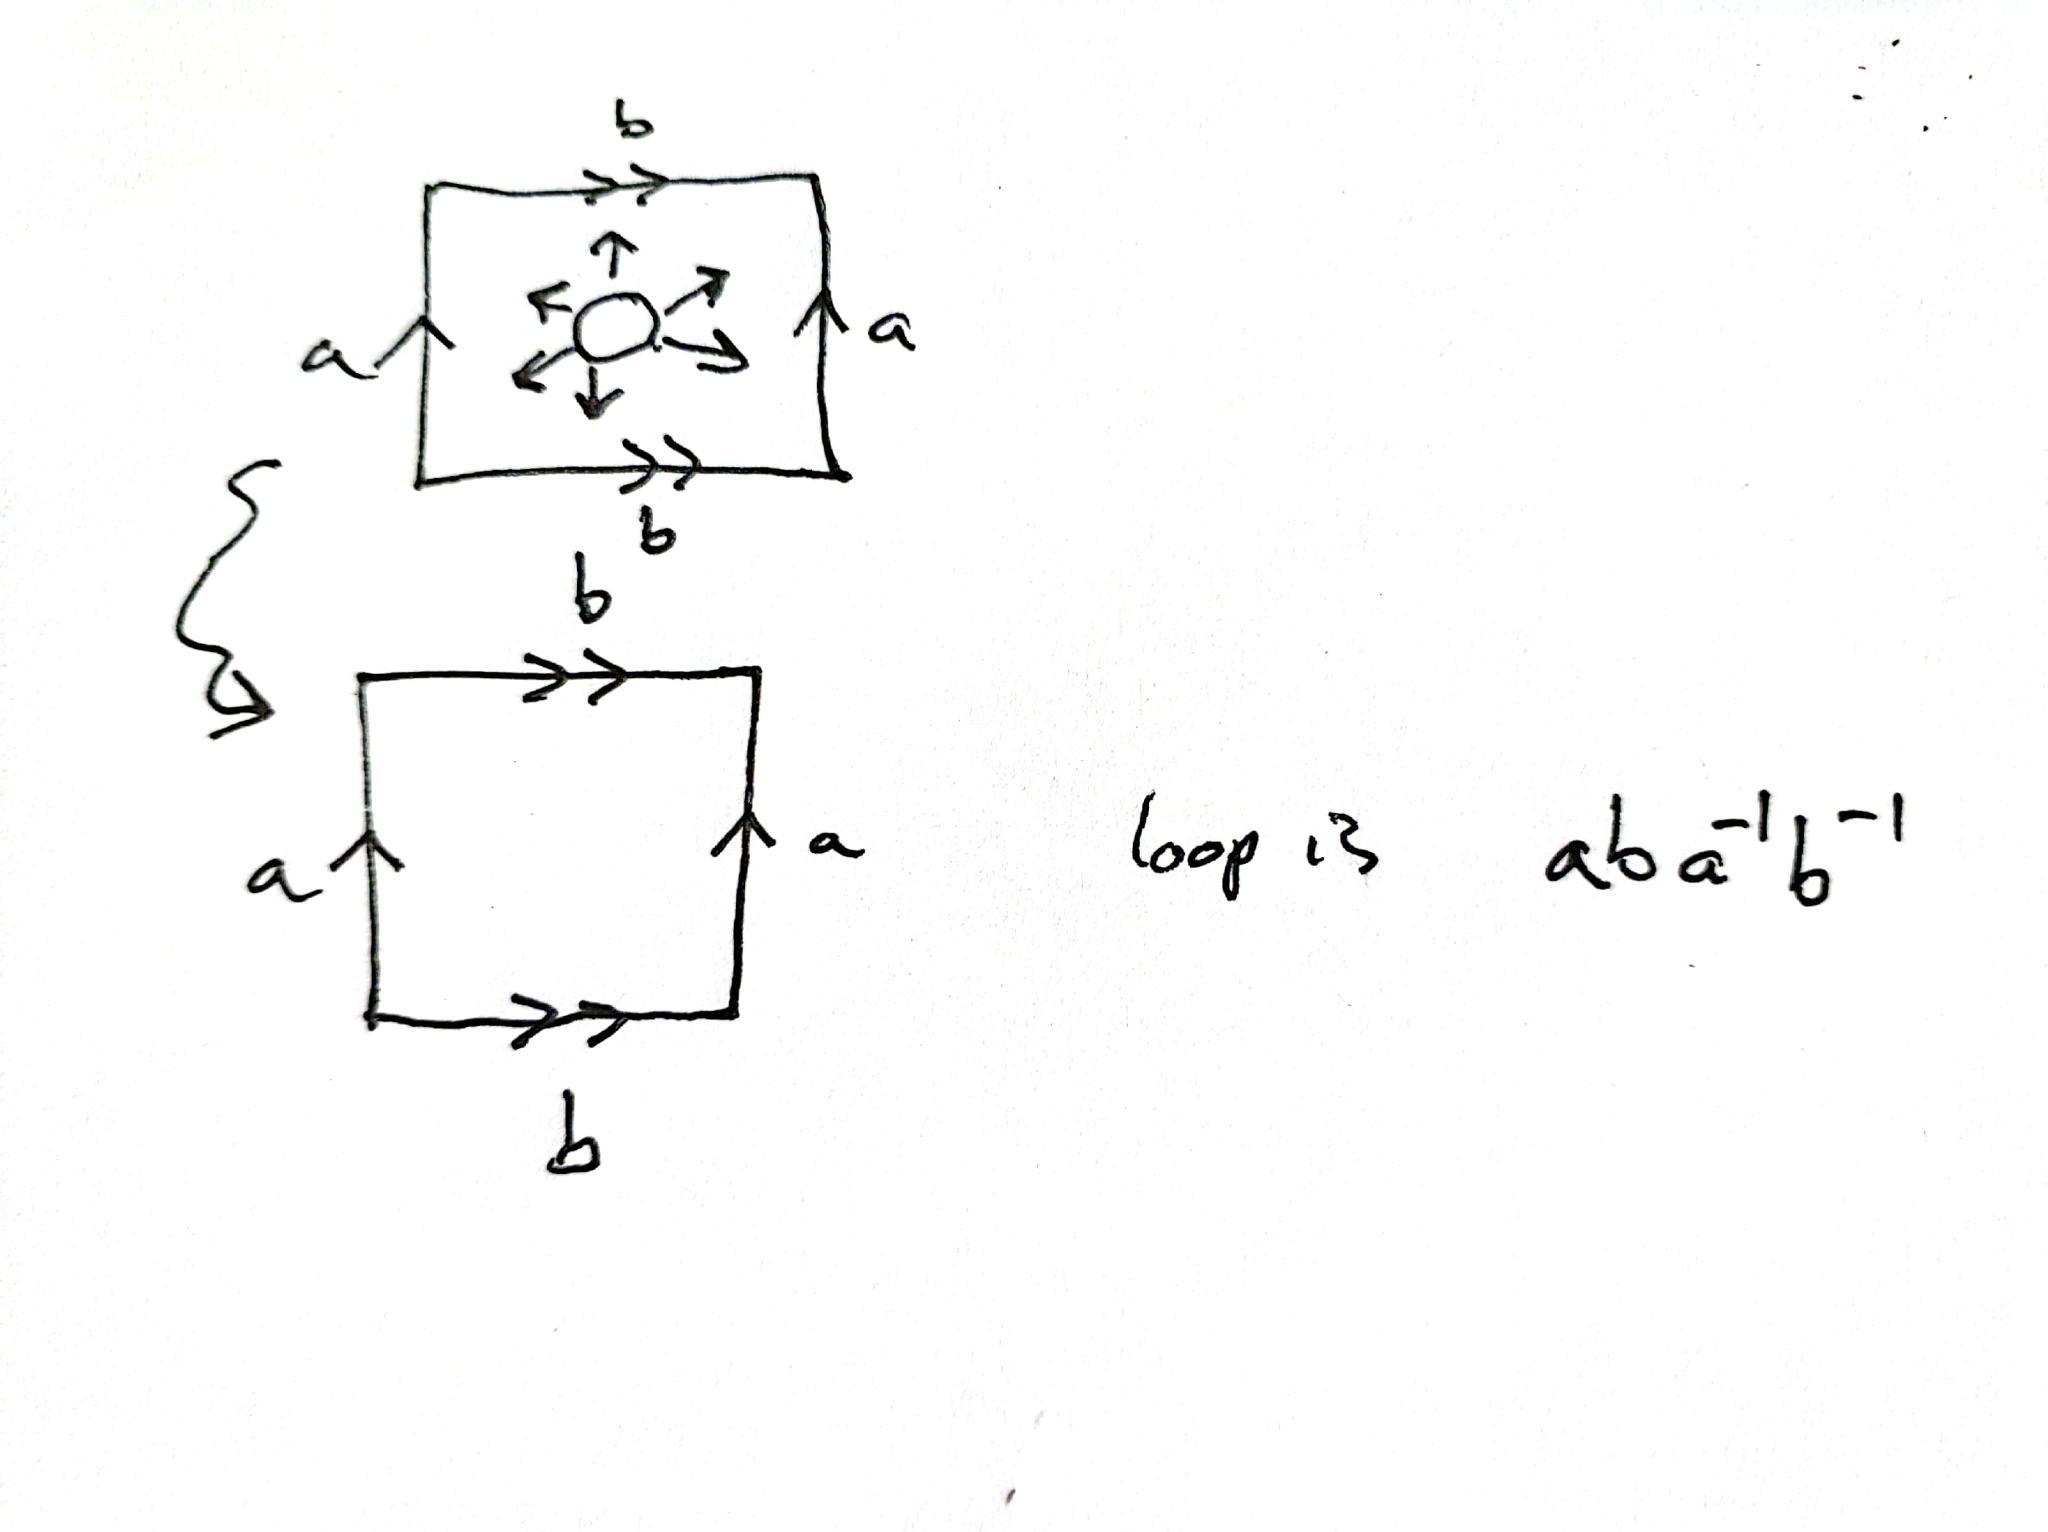
\includegraphics[width=0.6\textwidth]{12.jpeg}
          \label{fig:12-png}
      \end{figure}
      So, letting $a,b$ be the generators for the fundamental group of the left
      punctured torus, and $c,d$ the generators for the fundamental group of
      the right punctured torus, van Kampen gives that the fundamental group of
      the double holed torus is the free product
      $\left( \mathbb{Z} * \mathbb{Z} \right) *
      \left( \mathbb{Z} * \mathbb{Z} \right) \cong *_{4} \mathbb{Z}
      $ generated by $a,b,c$ and  $d$ with
      the relation
      $ab a^{-1}b^{-1} = cdc^{-1}d^{-1}$.
      So denoting the commutator of $x$ and $y$ by
      $\left[ x,y \right] = xyx^{-1}y^{-1}$, we get that the fundamental group is
      \[
      \langle a,b,c,d  \mid \left[ a,b \right] = \left[ c,d \right] 
       \rangle 
       = \langle a,b,c,d  \mid \left[ a,b \right] \left[ d,c \right]  \rangle.
      \] 
      Suppose instead we divide the torus into a disc and the closure as shown
      below (the identification space can e.g. be found in Hatcher page 5)

      \begin{figure}[H]
          \centering
          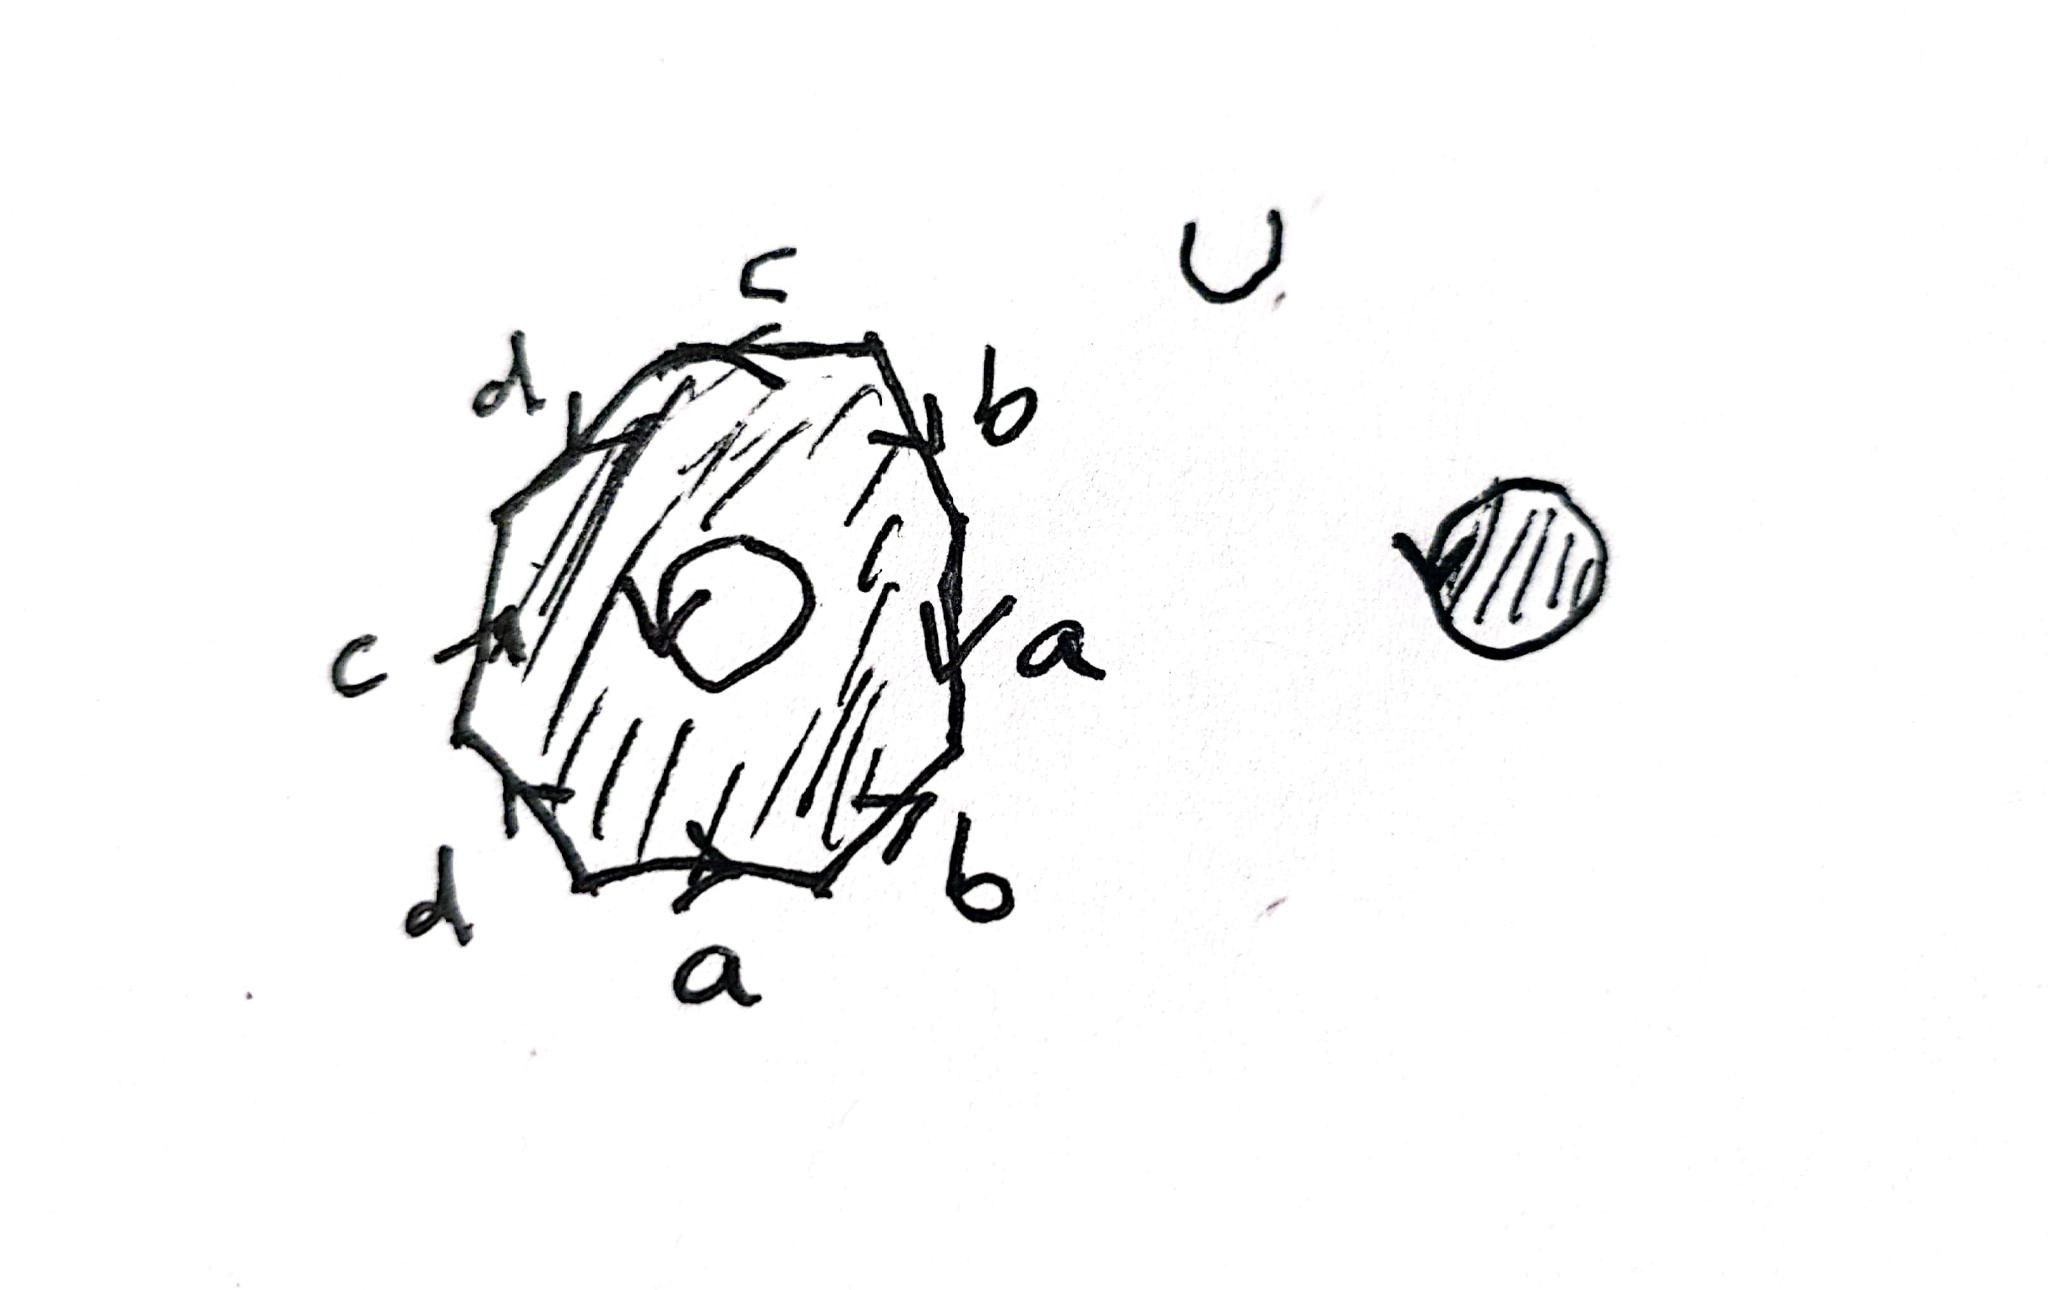
\includegraphics[width=0.5\textwidth]{13.jpeg}
          \label{fig:13-jpeg}
      \end{figure}
      
      Let $\left| J \right| $ denote the complement of the disc and
      $\left| K \right| $ the disc. Then
      $\left| J \cap K \right| $ is a circle again.\\
      Let $p$ denote a vertex on $\left| J \cap K \right| $ (interpreting
      it as a simplicial complex).\\
      Now, $\left| J \right| $ is clearly deformation retractable to the
      outer loop  $bab^{-1}a^{-1}dcd^{-1}c^{-1}$ by the projection from the
      center of the hole where the disc was removed. By the following figure,
      this outer loop is the identification space for the one-point union of
      4 circle, $\bigvee_{i=1}^{4}S_i^{1}$ :

      \begin{figure}[H]
          \centering
          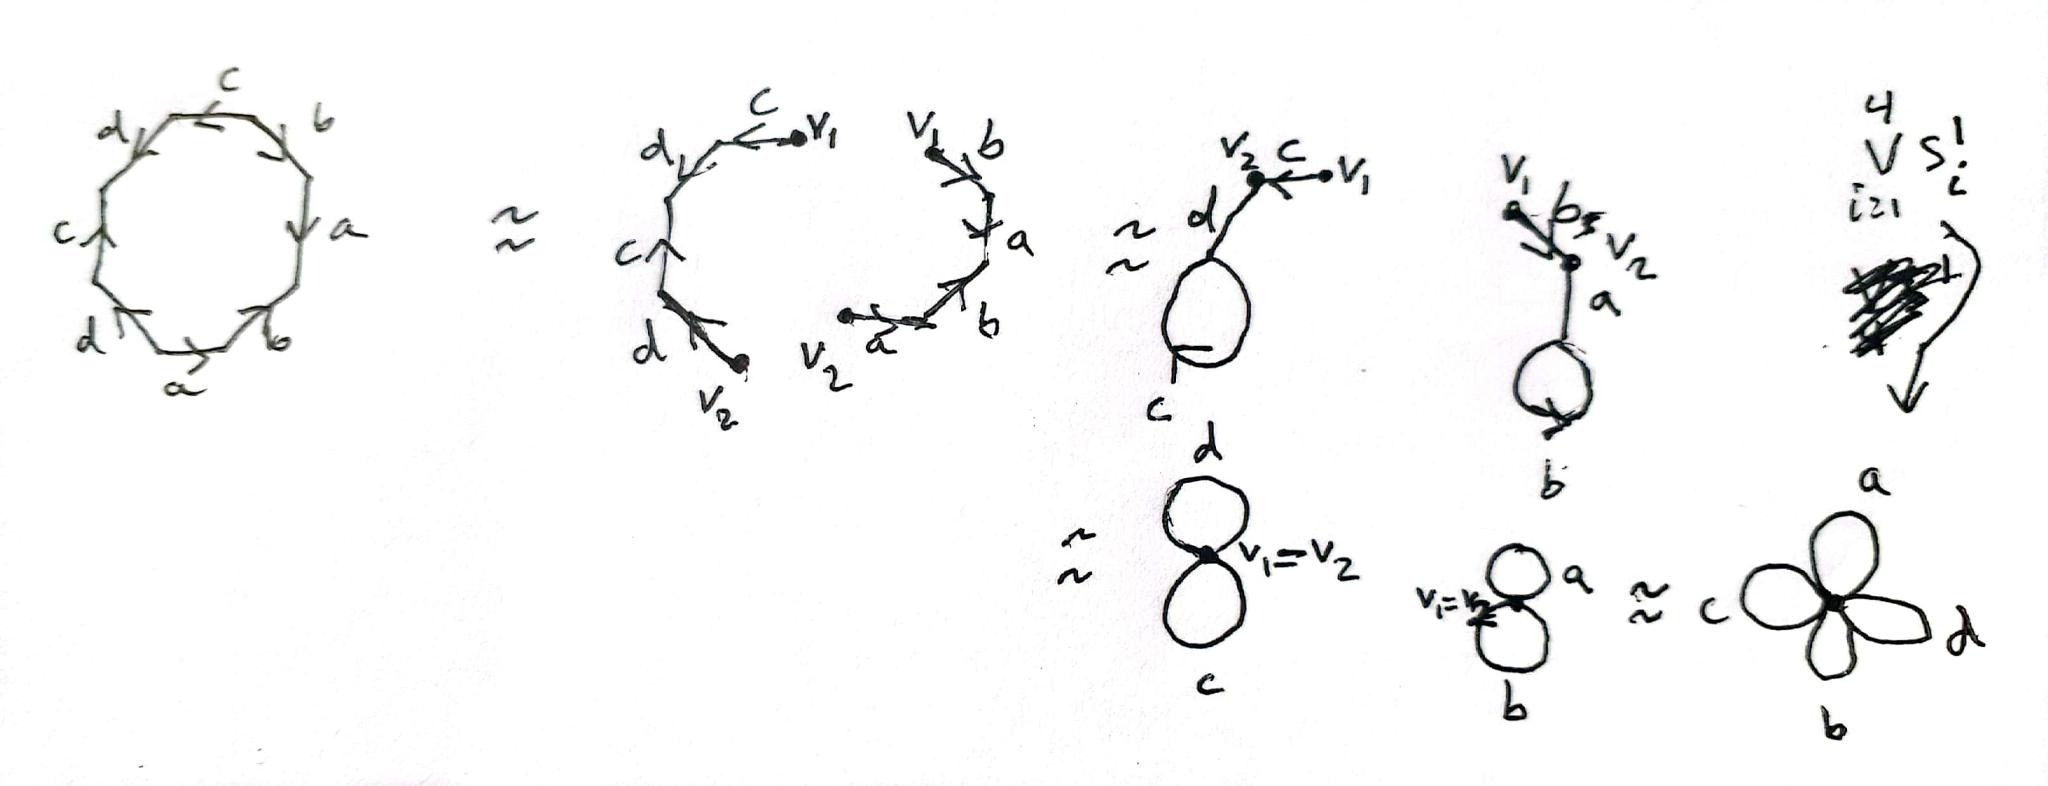
\includegraphics[width=1\textwidth]{14.jpeg}
          \label{fig:14-jpeg}
      \end{figure}

      Thus the fundamental group 
      $\pi_1 \left( \left| J \right| , p \right) $ is isomorphic to
      $\pi_1 \left( \bigvee_{i=1}^{4} S_i^{1} \right) $ which is isomorphic to
      the free group on four generators
      $*_{i=1}^{4} \mathbb{Z}_i$ by example 1 on page 136.\\
      Now, $\left| K \right| $ being a disc has trivial fundamental group as it
      is convex. The inclusions
      $ \left| J \right|\to \left| J \cup K \right|  $ and
      $\left| K \right| \to \left| J \cup K \right| $ thus identify the loop
       $ba b^{-1}a^{-1} dc d^{-1}c^{-1} = 
       \left[ b,a \right] \left[ d,c \right] $ and
       the trivial loop. Thus we recover by van Kampen, that the fundamental
       group of the double torus is
       \[
       \langle a,b,c,d  \mid 
       \left[ b,a \right] \left[ d,c \right] \rangle 
       \] 
       which was the same group that we got in the first part of the problem
       (b and a interchanged, however, this doesn't affect anything).\\
       \linebreak
       \textbf{23:} Let $X$ be a path-connected triangulable space. How does
       attaching a disc to $X$ affect the fundamental group of $X$?\\
       \linebreak
       \textit{Solution:} 
       We may suppose $X = \left| K \right| $ since the following proof is
       topologically invariant, and that $\left| K \right| $ has simplexes of
       dimension at most $2$ by example 3 on page 136. Since
       $\left| K \right| $ has a finite number of simplexes, 
       we can take a small $\varepsilon$-neighborhood of
       the image of the attaching map, call it 
       $f  \colon S^{1} \to X$, which is path connected and deformation
       retracts
       onto a circle or a point - depending on whether $f$ attaches along
       a loop, edge or a point. Now, by choosing a point
       $p$ on the image of $f$, van Kampen gives that the fundamental group
       of $\left| K \cup_f D \right| $ with respect to $p$ is
       $\pi_1 \left( \left| K \right|, p \right) * \pi_1 \left( D, p  \right)
       / N$ where $N$ is the normal subgroup formed by equating the inclusion
       of the circle $f \left( S^{1} \right) $ in each fundamental group. When
       included in $\pi_1 \left( D,p \right) $, it is nulhomotopic as $D$ is
       convex, and when included in $\pi_1 (X, p)$, it is simply
       the loop $t \mapsto f \left( e^{i \theta + 2 \pi i t} \right) $ with
       $f\left( e^{i \theta} \right) = p$. So since $\pi_1 \left( D,p \right) 
       $ is the trivial group, we get that attaching a disc to $X$ simply
       makes the loop $t \mapsto f \left( e^{i \theta}+ 2 \pi i t \right)
       $ homotopic to the trivial loop at $p$ in
       $\pi_1 \left( X,p \right) $.\\
       \linebreak
       \textbf{24:} Let $G$ be a finitely presented group. Construct a compact
       triasgulable space which has fundamental group $G$.\\
       \linebreak
       \textit{Solution:} For $G$ to be a finitely presented group means that
       $G$ is of the form
       $\langle S  \mid  R \rangle $ such that
       $S$ and $R$ are finite, so we can write
       \[
       G = \langle x_1, x_2, \ldots, x_n  \mid  r_1, r_2, \ldots, r_{m}
   \rangle. \]
       
       Now, as in example 1 on page 136, suppose we take
       $\bigvee_{i = 1}^{n} S_i^{1}$ which is triangulable as
       the one-point union of $n$ triangles like in figure 6.13. Like in that
       example, we can take a maximal tree $T$ which will consist of all
       edges connecting the central vertex/point to every other vertex,
       together with all the vertices. The fundamental group of this space is
       by the example isomorphic to $G(K,L)$ where
       $K$ is the triangulation of $\bigvee_{i=1}^{n} S_i^{1}$ and
       $L$ is the simplicial complex corresponding to the tree. Thus
       $G(K,L)$ consists of $g_{i,i+1}$ for the $i$ such that
       $v_i$ and $v_{i+1}$ are the endpoints of an edge in
       $K - L$ with an enumeration as in figure 6.13. This is precisely
       $\langle g_{1,2}, g_{3,4}, \ldots, g_{2n-1,2n} \rangle $. Now, we have that
       $r_i$ represents some loop in this interpretation of
       $G(K,L)$, namely, a relation of the form
       $g_{\alpha_1, \alpha_1 +1}^{\varepsilon_1} \ldots x_{\alpha_k,
       \alpha_k +1}^{\varepsilon_k}$ 
       corresponds the loop
       $E_{a_1} a_1 (a_1+1) E_{a_1 +1}^{-1} 
       E_{a_2} a_2 (a_2 +1) E_{a_2 +1}^{-1} \ldots
       E_{a_k} a_k (a_k+1) E_{a_k + 1}^{-1}$ in
       $E(K,v)$.\\
        \linebreak
       Now, letting
       $\alpha_i  \colon S^{1} \to \left| K \right| $ correspond to the kiio
       $r_i$ given above (we can let it map from $S^{1}$ without loss of
       generality) then since
       $K$ is path-connected and triangulable, we get from problem 23 that
       attaching a disc along $\alpha_i$ to $K$ will make the  loop
       $r_i$ nulhomotopic. Thus, we get that
        \[
       G = 
       \langle x_1, x_2, \ldots, x_n
        \mid  r_1, r_2, \ldots, r_m  \rangle 
       =
       \langle g_{1,2}, g_{3,4}, \ldots,
       g_{2n-1, 2n} \rangle \cup_{\alpha_1} D \cup_{\alpha_2} D
       \cup_{\alpha_3} \ldots \cup_{\alpha_{m}} D
       \] 
       

       




























\end{document}
